% !TeX root = thesis.tex
\documentclass{master_thesis}
\addbibresource{refs.bib}

\begin{document}

\section{Research}

\todo{Come up with a list of things that should be tested manually, based on my case study}

The research conducted for this thesis can be divided into 6 steps:

\begin{enumerate}
	\item Researching automated testing tools
	\item Pre-case study questionnaire
	\item Setting up automated testing tools in Pipedrive's component library
	\item Manual accessibility audit
	\item Comparing manual and automated testing results
	\item Post-case study questionnaire
\end{enumerate}

The first thing was to look at different automated accessibility tools that are available, test them out and see what would best fit our purpose. The tool needed to be easy to use for everyone and not block development. The next step was to send out a questionnaire to better understand the current approaches toward accessibility among the people who work on it the most. After that, an automated accessibility tool was added to the component library repository and announced in relevant channels to raise awareness about it.

In parallel to observing how the tool was being used I conducted a manual accessibility audit together with 3 designers on the same component library. These results were then compared with the automated testing results that we got from the same version of the library. As the last step, I sent out a questionnaire to gather information about how the tool had been adopted. To get more details I also interviewed some developers and designers I knew had used the tool during that period.

Pipedrive has been developing a sales \ac{crm} using mostly typescript and React. Accessibility has never been a high priority and at this point, it would not be very easy to get started. We have a design system and a React-based component library to keep the look and \ac{ux} consistent. This seemed like a good place to start solving accessibility issues. The library is used widely in the company and developers from different teams contribute to it. If a button in the reusable library gets fixed, most of the buttons in the web app that our customers use should be improved.

This should not be taken as a way to solve all accessibility problems but as a good first step to get started. Making changes in a reusable \ac{ui} library should have a wide impact on the product's overall accessibility and without establishing a basic level of accessibility there, it would be difficult to start testing individual pages of the final product.

\subsection{Current state of awareness about accessibility in Pipedrive}

First, I sent out a survey in our company's Slack channels (see figure \ref{fig:slack-message}) to understand what is the knowledge and general approach to web accessibility in the company. It was shared in 4 channels to reach people who are most likely to be dealing with accessibility, our component library and who are invested in accessibility (see more details in table \ref{table:survey-shared}).

\begin{table}[H]
	\centering
	\begin{tabular}{|l|l|}
		\hline
		\textbf{Channel members or theme} & \textbf{number of members}  \\
		\hline
		Front end developers  & 212  \\
		\hline
		Dedicated to our component library  & 124  \\
		\hline
		Designers  & 73  \\
		\hline
		Accessibility channel  & 31  \\
		\hline
	\end{tabular}
	\caption{List of all the channels the survey was shared in.}
	\label{table:survey-shared}
\end{table}

Some people might also be on more than one of these channels. The aim was to reach people in the company who would be most likely to be using these tools and contribute to the library. There were 7 questions and some of them also included a field for free text to give more details on the subject if they wanted.

\begin{figure}[H]
	\centering
	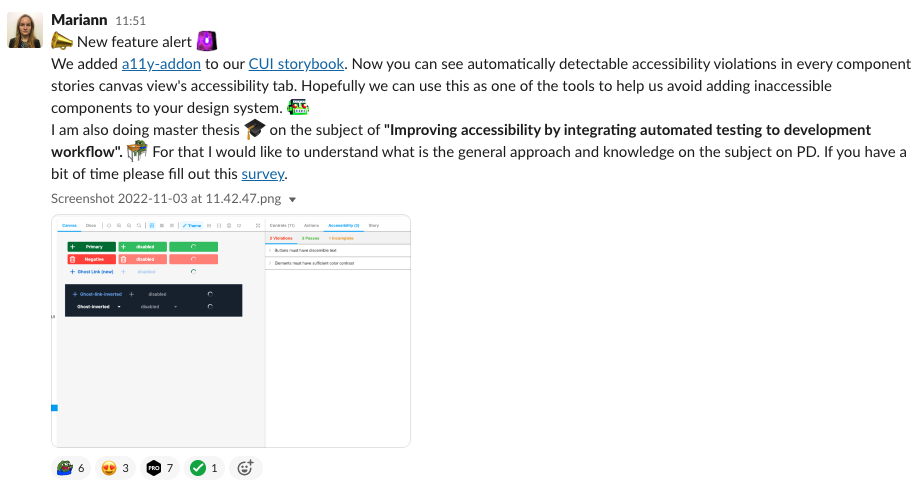
\includegraphics[width=\textwidth]{img/survey.png}
	\caption{Message in company Slack announcing adding accessibility tool and inviting people to reply to the survey.}
	\label{fig:slack-message}
\end{figure}

In total, 20 people replied to the survey - 6 designers and 14 developers, including one engineering manager. This does not give a full overview of the company, but it should give a good insight into the general opinions regarding accessibility. Likely, developers and designers that are more involved with our component library and/or interested in accessibility were more likely to respond.

\begin{figure}[H]
    \centering
	\begin{subfigure}{0.5\textwidth}
		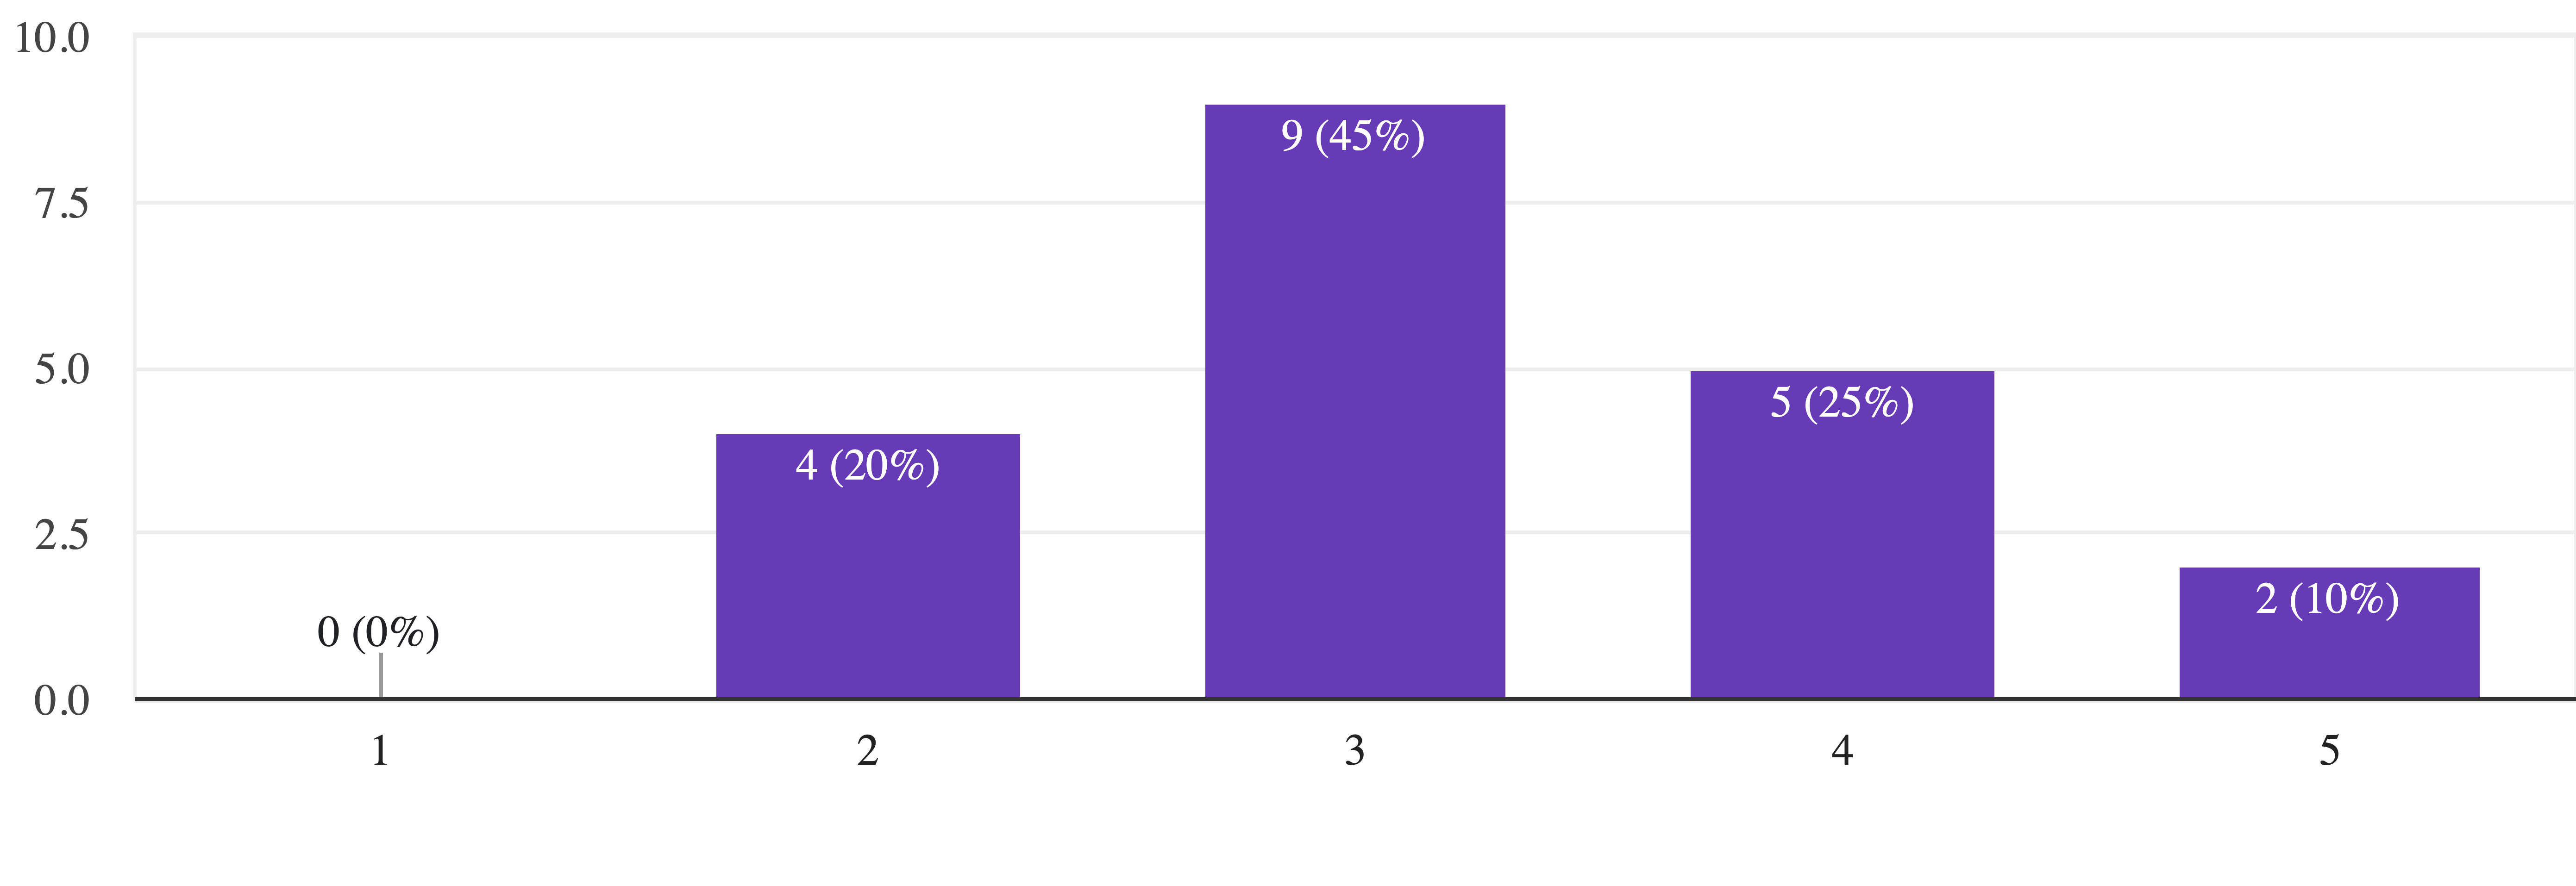
\includegraphics[width=\textwidth]{img/a11y-knowledge.png}
		\caption{Pre-case study survey: How much do you know about accessibility (standards, best practices, importance, testing)? 1- "Almost no knowledge" to 5 - "I have very good knowledge" }
		\label{fig:a11y-knowledge-current}
	\end{subfigure}
	\hspace{0.05\textwidth}
	\begin{subfigure}{0.4\textwidth}
		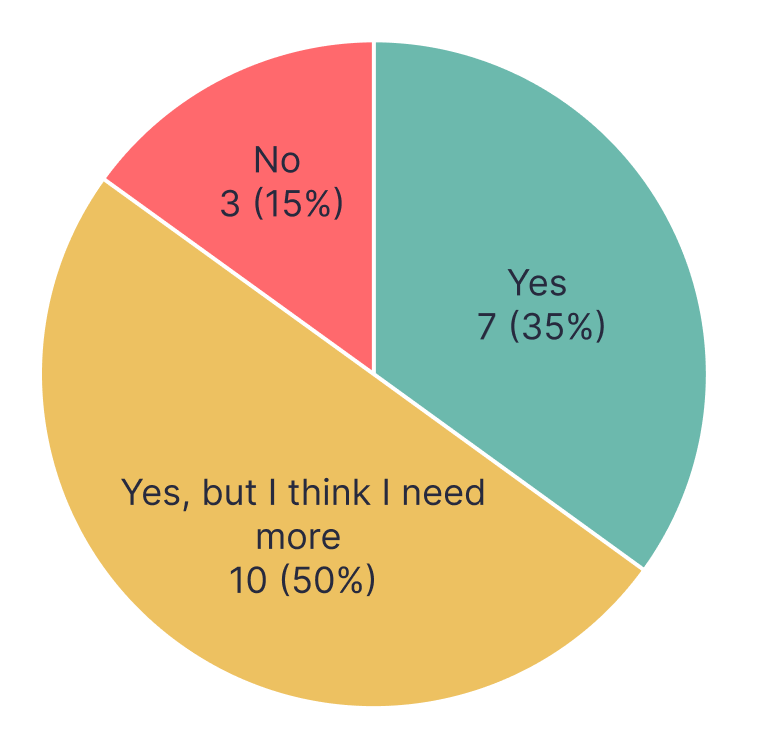
\includegraphics[width=\textwidth]{img/a11y-resources.png}
		\caption{Do you know where to find resources
		about accessibility standards? (no one chose the 4th option "No I don't think I need them") }
    	\label{fig:a11y-resources}
	\end{subfigure}
	\caption{Accessibility knowledge in Pipedrive}
    \label{fig:a11y-knowledge}
\end{figure}

The results show that 10\% of people who responded think their knowledge of accessibility is very good, while most think that their knowledge level is average (see Figure \ref{fig:a11y-knowledge-current}). 35\% of responders know where to find resources about accessibility standards, 15\% don't know and 50\% know, but think they need more (see Figure \ref{fig:a11y-resources}).

\begin{figure}[H]
    \centering
	\begin{subfigure}{0.45\textwidth}
		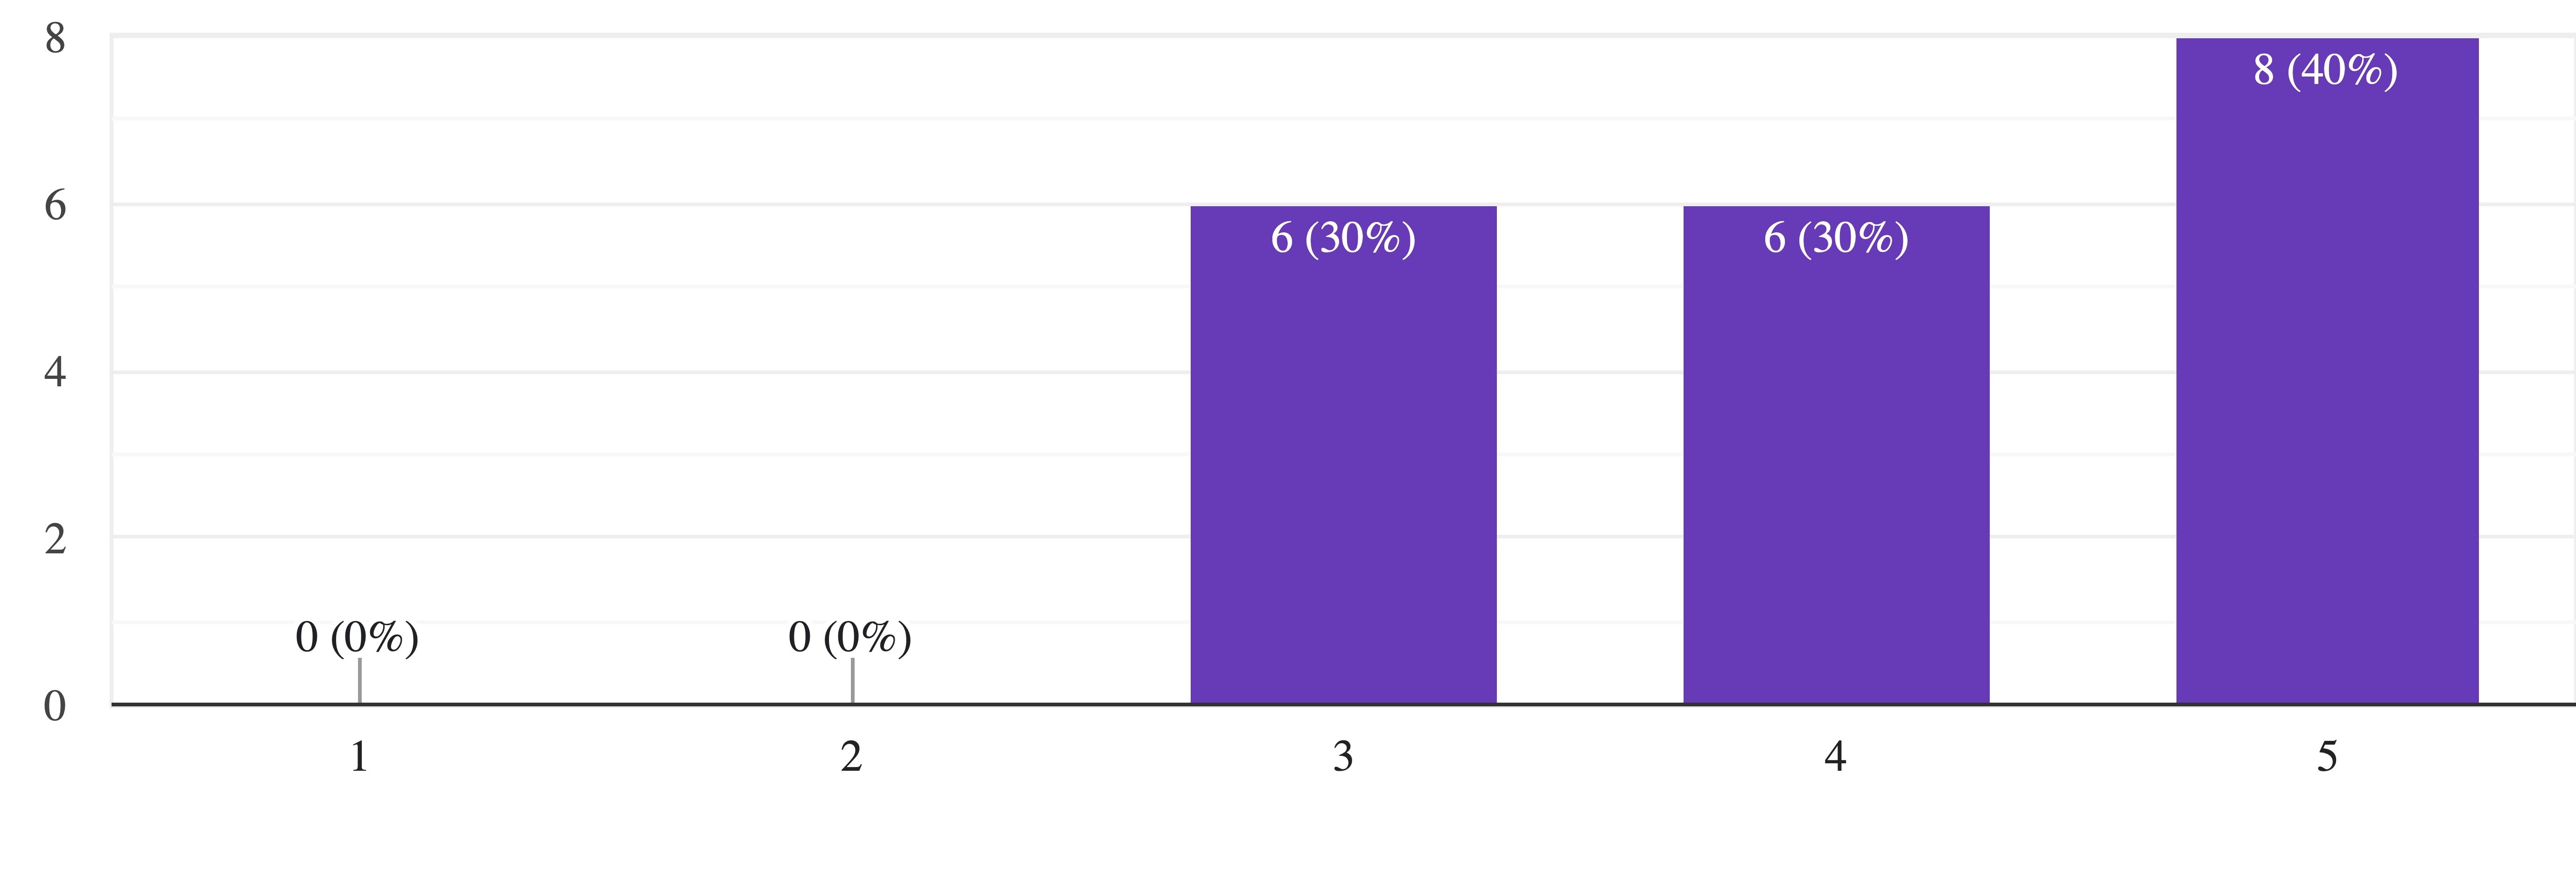
\includegraphics[width=\textwidth]{img/a11y-priority.png}
		\caption{Do you think accessibility is a priority in our company? 1-No not at all to 5-Yes very much \\
		\\
		\\}
	\end{subfigure}
	\hspace{0.05\textwidth}
	\begin{subfigure}{0.45\textwidth}
		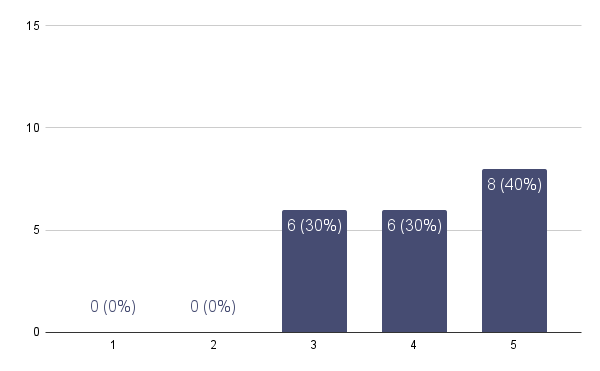
\includegraphics[width=\textwidth]{img/a11y-goals.png}
		\caption{Do you think we should prioritize following accessibility standards (like \ac{wcag}, EN 301 549) in our product? 1- "No I think they are irrelevant for Pipedrive customers" to 5 - "Yes I think following accessibility standards should be a high priority" }
	\end{subfigure}
	\caption{Priority of accessibility in Pipedrive}
    \label{fig:a11y-priority}
\end{figure}

Most people who replied to the survey don't think accessibility is being prioritized in Pipedrive and at the same time, most of them think we should be putting more focus on following common accessibility standards (see Figure \ref{fig:a11y-priority}). They elaborate a bit more about what they think the reasons behind this are. Accessibility has always been at the end of our priorities and there is no clear company-wide strategy on how to manage and improve it. There has never been a dedicated project manager to bring focus to it
and right now developers and designers are the ones that seem to be responsible for it. Two people also mentioned that the priority might be low because as a private service, Pipedrive does not have a legal obligation to comply with any specific accessibility standard. Two people think that it would not affect Pipedrive's customers much.

It seems like the biggest obstacle to improving the accessibility of Pipedrive is the lack of knowledge about the business impact. More knowledge would help prioritize solving these problems. There is a lot currently that could be improved, but in my opinion implementing a way of continuously testing for at least some basic issues from the beginning of all new developments would help to ensure that the technical debt related to accessibility would not grow to be even bigger. There were several comments in the free text sections expressing saying they appreciate this subject being brought to focus and even some offering to help.

\subsection{Adding automated accessibility tests to component library}
The next step was adding some automated tests to our component library's development workflow and observing their usefulness. The aim was to find something that we can integrate easily and that does not have a steep learning curve or add unnecessary complexity.

We use Storybook as the component explorer for our reusable component libraries development. It is open-source software for \ac{ui} development that allows teams to work on one component at a time \citep{storybook}. It allows us to render isolated \ac{ui} components without integrating them into the final product right away. Our developers use it to test out the components they are developing locally. We also have a version of Storybook with all the components available for anyone in the company to see. As this is the first place where elements are rendered it seemed logical to try to find a way to start testing them there.

Each component has stories – examples of how the component would be used in real life. These stories will be rendered in a browser inside Storybook \ac{ui}. It also has a sidebar for navigating between different examples, and controls for additional tools and documentation. This means it would not be very easy to use a browser extension for accessibility testing because it would also test the Storybook \ac{ui} around the actual relevant example.

\begin{figure}[H]
	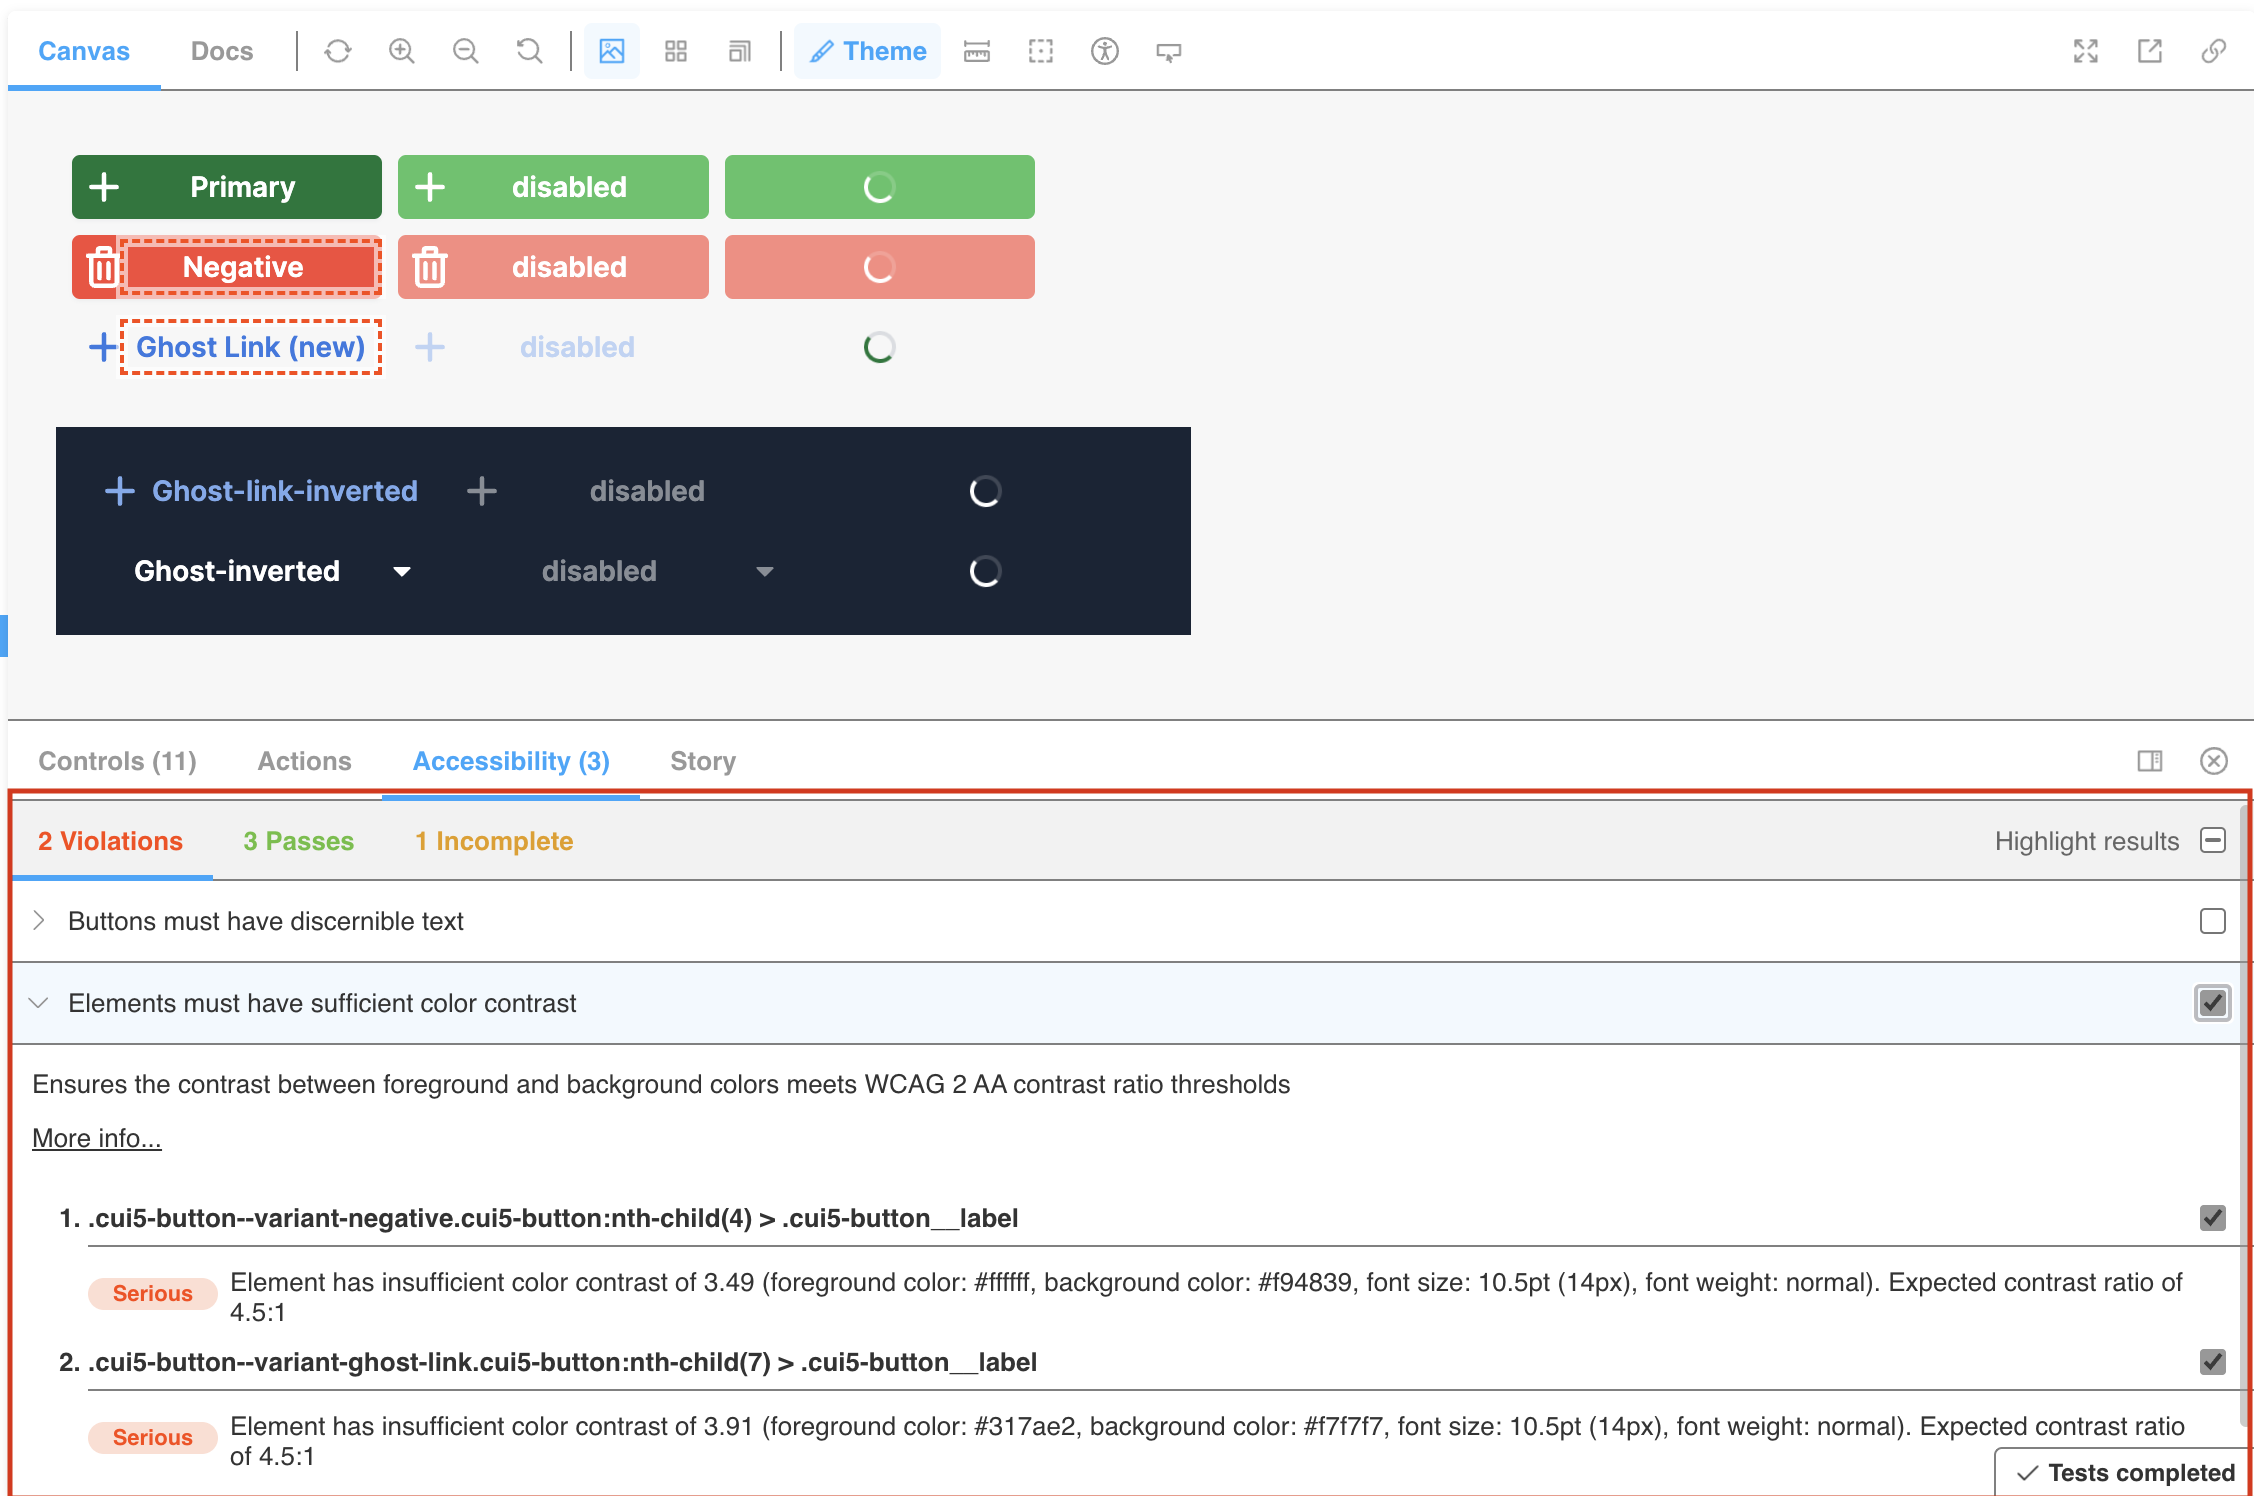
\includegraphics[width=\textwidth]{img/addon-a11y.png}
	\caption{Accessibility add-on for Storybook (addon-a11y)}
	\label{fig:addon-a11y}
\end{figure}

Storybook has a wide ecosystem of add-ons and one of them is addon-a11y (see figure \ref{fig:addon-a11y} ). It uses Deque's axe-core to audit the \ac{html} rendered for an isolated component \citep{addon-a11y}.

Axe-core is an accessibility testing engine for websites and other \ac{html}-based user interfaces \citep{Deque2023}. It includes \ac{wcag} 2.0 and 2.1 on levels A and AA and it has a coverage of about 20-30\% if you calculate it in a commonly used way, but they claim it to be 57\% according to their new and improved calculation method. This has been explained in more detail in the Automated accessibility testing chapter.

This seemed like the best solution in our situation so addon-a11y was added to our component library’s Storybook. The tool is visible in the add-ons sidebar of every component example. It shows all the checks that the component has passed, all the violations that were found and any issues that could not be checked and might need manual testing. Every rule listed there also has reference to the \ac{html} node that had the violation, explanation and links to the Deque webpage with examples. This should be very useful in understanding and fixing these issues.

The rules format that axe-core uses is developed by Deque Systems and is an adoption of the \ac{act} rules format developed by \ac{wai} \citep{Fiers2017}. They have a set \ac{wcag} that can be evaluated in a fully automated way. They are divided by \ac{wcag} standards version (2.0, 2.1, 2.2) and Level (A \& AA, AAA) and they also have some rules for best practices in the industry that improve the user experience but might not conform to \ac{wcag} success criterion \citep{Fiers2023}.

I used Storybook-a11y-report \citep{Karube2020} to generate a report of all the violations in the whole component library. It went through all the examples and ran the same tests as addon-a11y to generate a summarized report. The final report links back to each component's story where you can see the example and addon panel with all the information mentioned before. \todo{add the report to Appendices and reference it here.}

To get some data that could be compared with the results from manual testing, I went through all the examples and extracted the following info for each component:

\begin{itemize}
	\item How many occurrences of the component are there in the accessibility violations report? One issue might have been reported multiple times because most components have several examples and issues might be reported in each of them.
	\item How many unique issues does the component have? Most components have more than one story. I opened the example and went through all the violations in all the stories and counted unique ones.
	\item How many passed checks does the component have? This together with violations will show how many things were tested for each component. Same method as in the previous item - all unique passed checks in all the stories for that component.
	\item How many of these checks are valid? I looked at the example and only counted passed issues that are valid and relevant to the component that the example is about.
\end{itemize}

\subsection{Manual accessibility audit}

The second part was conducting a manual accessibility audit of the same library to get a better overview of all the issues. This would also allow me to compare the results of the manual testing with the automatically generated test report to determine what are the tool's strengths and weaknesses and if testing isolated components poses any limitations.

\subsubsection{Methodology for manual audit}
We used Storybook to render an isolated preview of each component.
The accessibility add-on had already been installed, and we looked at the violations reported there also. We worked in a team of 4 people - 3 designers and 1 developer. We created a task for each component - 53 tasks in total.

Everyone worked individually and each morning we had a quick meeting to discuss any questionable issues. Each evaluator checked violations in the accessibility add-on panel, using a keyboard, and also a screen reader to navigate. Each component had 1 or more examples and we looked at as many as we thought relevant to get a good overview.

At the beginning of the audit, we tested an add-on in Storybook for mocking a screen reader \citep{Lara}. It had the option to show the output that the screen reader would play as audio, as text. Initially, it seemed like a convenient solution with rather reliable results, but further investigation revealed that the output was very different from what an actual screen reader would say.

For the rest of the audit, we used VoiceOver - the built-in screen reader for Apple products, because our work computers are MacBooks and VoiceOver was conveniently available for us to use. There was an initial learning curve, but after that, it went quite smoothly. All the components that had already been tested with the faulty add-on were reviewed again using VoiceOver.

The audit results were documented in a table. We used the barrier walkthrough method where the barriers we focused on were defined by how the user interacts with the webpage and looked at what issues different types of users might encounter. We separated them into 3 sections:
\begin{enumerate}
	\item Mouse user issues - using a mouse to interact with the page
	\item Keyboard user issues - using only a keyboard to do the same things
	\item Screen reader user issues - trying to do the same things and getting the same information while only using a screen reader
\end{enumerate}

We see this separation as a good way to prioritize fixing the issues in the future. The mouse user is the user we are considering in all of our development currently. The issues they would encounter should be the most critical. This category includes a lot of visual, color contrast, and click target size issues.

The second type of user would encounter all the issues from the first category plus everything that is unusable for them by using a keyboard. We took the functionalities that the user should be able to use with a mouse and tried to use them with a keyboard only.
\review{Mari-Ell: But it is OFTEN the case that screen reader works better than keyboard}

The third user was imitated using a screen reader. The prerequisite for this was keyboard accessibility - if it was not usable with a keyboard then most likely it would not be usable by a screen reader.

In real life, these 3 types of users might not be so clearly separated and many issues would affect all types of users, but as the intention was to come out of the audit with an actionable list, we needed to prioritize the issues while we found them in order of severity and current customer impact. These categories also mostly depend on each other, so it would make sense in most cases to start by solving mouse user issues, then keyboard user issues and then screen reader user issues.

\end{document}